\documentclass[a4paper,11pt]{article}
\usepackage[T1]{fontenc}
\usepackage[utf8]{inputenc}
\usepackage{lmodern}
\usepackage{hyperref}
\usepackage{amsmath}
\usepackage{amssymb}
\usepackage{xcolor}
\usepackage{graphicx}
\usepackage{wrapfig}
\usepackage{caption}
\usepackage{multicol}

\hypersetup{
  colorlinks=true,
  linkcolor=gray,
  urlcolor=blue
}

\title{Parallel Solution of Laplace's Equation}
\author{Leo Unbekandt}

\begin{document}

\maketitle
\tableofcontents

\begin{abstract}
  The main goal of this work is to develop a parallel way to solve numerically Laplace's Equation by using OpenMPI,
  and to analyze how this process accelerates the computation compare to the serial way to do, and how exact are the
  results compare to the analytical solution. The using method in this project must have been Jacobi with red-black
  ordering. However there is no interest in doing red-black ordering with Jacobi as the old matrix has to be kept in
  memory, that's why I've decided to use Gauss Seidel method associated with red-black ordering.
  
  The complete source code of this project may be found on Github: \url{https://github.com/Soulou/HPC_Assignment}
  It includes the analytical, the serial and the parallel methods, and additionaly the \LaTeX \hspace{5pt} source code of this
  report.
\end{abstract}

\section{The analytical solution}
\subsection{Solving the equation by using Fourier series}

Finding the analytical solution basically consists in solving:
2$$\frac{\partial^2 \phi}{\partial y^2} + \frac{\partial^2 \phi}{\partial x^2} = 0 \hspace{2em} x \in [0,1], y \in [0,1]$$

\noindent The homogeneous boundary conditions are:
$$\phi(x,0) = 0 \hspace{3em} \phi(x,1) = 0 \hspace{3em} \phi(1,y) = 0$$

\noindent The inhomogeneous boundary condition is:
$$\phi(0,y) = sin^2(\pi y)$$

\noindent After separating the variables, $\phi(x,y) = X(x)Y(y)$, so Laplace's equation becomes:
$$\frac{1}{X}\frac{\partial^2 X}{\partial x^2} + \frac{1}{Y}\frac{\partial^2 Y}{\partial y^2} = 0$$

\noindent Let: $$\frac{1}{Y}\frac{\partial^2 Y}{\partial y^2} = - k^2 \Leftrightarrow Y(y) = A_1\cos(k y) + B_1\sin(k y)$$ 
So:
\begin{align*}
  \frac{1}{X}\frac{\partial^2 X}{\partial x^2} = k^2 \Leftrightarrow X(x) & = A_2\cosh(k x) + B_2\sinh(k x) \\
  Or: X(x) & = A_2\cosh(k (x-1)) + B_2\sinh(k (x-1))
\end{align*}

\noindent This second expression works better with $X(0) = 0$ as boundary condition. The result is:
$$\phi(x,y) = [ A_1\cos(k y) + B_1\sin(k y)][A_2\cosh(k (x-1)) + B_2\sinh(k (x-1))]$$

\noindent Thanks to our boundary conditions, it can be deduced that
$$Y(0) = 0 \Rightarrow A_1=0 \hspace{2em} Y(1) = 0 \Rightarrow k=n \pi \hspace{2em} X(1) = 0 \Rightarrow A_2 = 0$$

\noindent Finally:
\begin{align*}
  \phi_n(x,y) & = B_n \sin(n \pi y)\sinh(n \pi (x-1)) & for\hspace{5pt}n \in \mathbb{N}^{+*} \\
  \phi_n(x,y) & = \sum_{n = 1}^{\infty}{B_n \sin(n \pi y)\sinh(n \pi (x-1))} & (by\hspace{5pt}superposition)
\end{align*}

\noindent Thanks to the inhomogeneous boundary condition:
\[
  \phi(0, y) = \sum_{n = 1}^{\infty}{B_n sin(n \pi y)\sinh(-n \pi)}
\]
The Fourier coefficient is now $B_n \sinh(-n \pi)$:
\begin{align*}
  B_n \sinh(-n \pi) & = \int_{0}^{1}{\sin^2(\pi y)\sin(n \pi y)dy} \\
  B_n & = \frac{2(\cos(\pi n) - 1)}{\pi(n^3 - 4n)\sinh(-n \pi)}
\end{align*}

\subsection{Implementation of the solution}
  The implementation has been done with the C programming language. The only constraint of using this language is
  that the result formula contains $\sinh(-n \pi)$. When $n$ gets bigger, a primitive variable type (double, long double)
  is not able anymore to have enough precision to compute correct results. This is why I've used the library
  GNU MPFR which is used to manipulate with high precision floating point numbers.
  
\subsection{Illustration of the analytical solution}

\begin{figure}[h!]
  \centering
  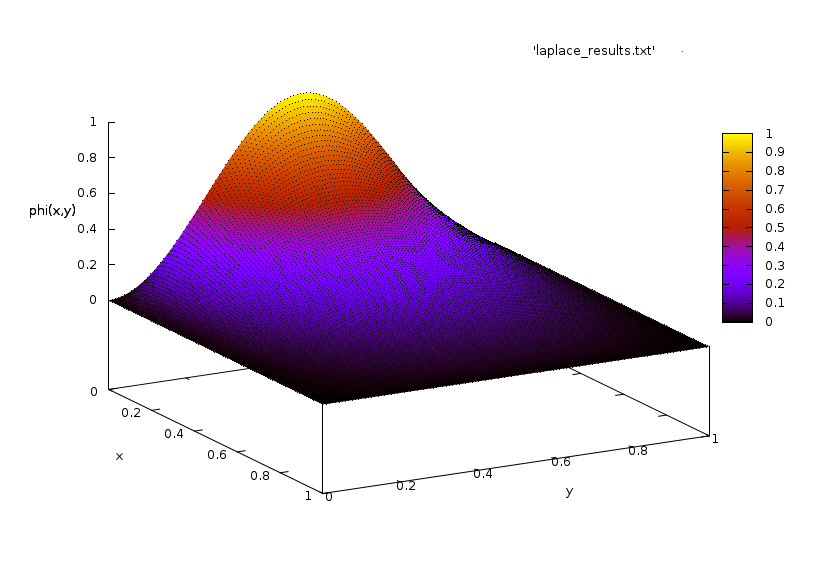
\includegraphics[width=0.8\textwidth]{images/analytical.png}
  \caption{Representation of $\phi(x,y)$ for a stepsize of 1/120}
\end{figure}

\clearpage

\section{The numerical solution - serial computation}
\subsection{Implementation}

\begin{wrapfigure}[13]{l}{0.45\textwidth}
  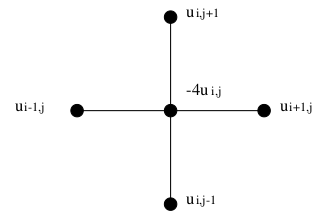
\includegraphics[width=0.45\textwidth]{images/gauss-seidel.png}
  \caption{Finite difference stencil}
  \label{fig:stencil}
\end{wrapfigure}

The implementation of Gauss-Seidel method consists in a successive number of iterations of the following formula:

$$\phi^{k+1}_{i,j} = \frac{1}{4}(\phi^{k}_{i+1,j} + \phi^{k+1}_{i-1,j} + \phi^{k}_{i,j+1} + \phi^{k+1}_{i,j-1})$$
$$i \in [2;k-1], j \in [2;k-1]$$

\vspace{1em}

As shown the figure~\ref{fig:stencil}, the current value is calculated from the four values which circle it.
This is really convenient to implement, because by iterating by line as it is showed in the following schema, when
the point $o22$ is calculated, $\phi^{k+1}_{i-1,j}$ and $\phi^{k+1}_{i,j-1}$ have already been defined because they have been
computed previously. Consequently eep a copy of the old matrix in memory, we can iterate
on in directly.
  
\begin{verbatim}
                 _____________________________
                |                             |
                | f   0   0   0   ...   0   0 |
                | f  n11 n12 n13  ...  n1k  0 |
                | f  n21 o22 o23  ...  o2k  0 |
                |                             |
                |                             |
                |           .........         |
                |                             |
                |                             |
                |                             |
                |_____________________________|
\end{verbatim}

Another important point, is the stopping condition. The following choice has been done: after each iteration 
the norm of the difference between the newly computed matrix and the previous one is compared to a certain tolerance
the user has to give as argument to the software. When this norm is close to 0, it means that the newly generated matrix is
not different anymore from the previous one, The algorithms stops iterating at the precise point.

\[
  ||\phi^{k+1} - \phi^{k}|| < \epsilon
\]

\subsection{Aspect of the results}

The results look similar as the results obtained in the analytical computation:

\begin{figure}[h!]
  \centering
  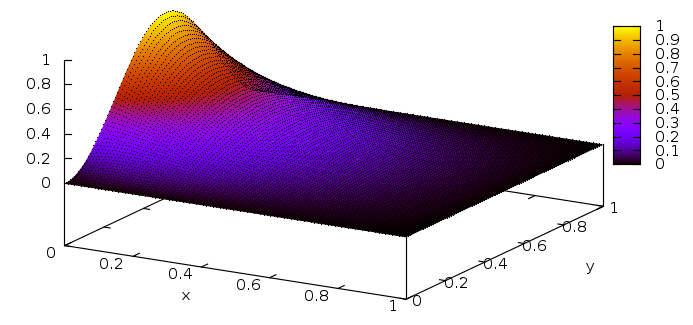
\includegraphics[width=0.85\textwidth]{images/serial-results.png}
\end{figure}

\subsection{Validation of the implementation}

To know if the results are accurate, the results of the numerical solutions are compared to he results of the analytical solution. In order to
achieve that, The small script: \texttt{diff\_results.rb} compares two result files by calculating the
difference of each $\phi(x,y)$ and finally printing the average difference in percents. The following table shows the difference
between the analytical implementation and the Gauss-Seidel serial version, for different sizes of domain and different error tolerances
\footnote{Data generated by: analytical\_serial\_diff.sh}.

\begin{itemize}
\item{N: Number of steps/size of the result matrix}
\item{\=e: Average error}
\item{t: convergence tolerance}
\end{itemize}

\begin{center}
\begin{tabular}{c | c | c | c | c}
N & \=e ,t = $10^{-2}$ & \=e, t = $10^{-3}$ & \=e, t = $10^{-4}$ & \=e, t = $10^{-5}$ \\
20 & 0.1822 & 0.1325 & 0.1234 & 0.1227 \\
40 & 0.2170 & 0.1086 & 0.0737 & 0.0708 \\
60 & 0.2626 & 0.1091 & 0.0554 & 0.0500 \\
80 & 0.3004 & 0.1171 & 0.0465 & 0.0388 \\
100 & 0.3206 & 0.1228 & 0.0421 & 0.0320 \\
\end{tabular}
\captionof{table}{Difference between analytical and serial solutions}
\vspace{1em}
\end{center}

There are different things observable in this table. First, whatever is the size of the domain,
the precision of the results is better when the tolerance is decreasing. Then, the results look accurate when the 
convergence tolerance is small enough. Actually when $t = 10^{-5}$ and $N \geq 60$, the numerical results are less
than 5\% different from the analytical one. Finally, the bigger the domain, the small the required
tolerance has to be to obtain good results. As a result, this way can be validated in order to measure the error and to detect the
convergence.

\subsection{Investigation of the rate of convergence}

This rate is expressed like that:

\[
  \frac{||\phi^{k+1}-\phi^{k}||}{||\phi^{k}-\phi^{k-1}||}
\]

It compares the previous error to the current one. In this case, it looks like the following
graph:

\input convergence_rate

At the beginning, the value is really low, because the error is decreasing fast, after a couple
hundreds iterations, the content of the result matrix begins to be more stable and more precise,
the is why the rate of convegence is approaching $1$. The bigger the asked precision, the closer
to $1$ will be the rate of convergence.

\clearpage  

\section{OpenMPI - parallel computation}

\subsection{Computational domain decomposition}

To divide a matrix, there are two main solutions:
\begin{itemize}
\item{Panels:
\begin{multicols}{2}
\begin{verbatim}
 ____________________
|      |      |      |
|      |      |      |
|      |      |      |
|      |      |      |
|      |      |      |
|      |      |      |
|      |      |      |
|      |      |      |
|______|______|______|
\end{verbatim}
\vspace{1em}
\begin{verbatim}
 ____________________
|                    |
|                    |
|____________________|
|                    |
|                    |
|____________________|
|                    |
|                    |
|____________________|
\end{verbatim}

\end{multicols}
}
\item{Squares:
\begin{multicols}{2}
\begin{verbatim}
 ____________________
|          |         |
|          |         |
|          |         |
|          |         |
|----------|---------|
|          |         |
|          |         |
|          |         |
|__________|_________|
\end{verbatim}

\begin{verbatim}
 ____________________
|      |      |      |
|      |      |      |
|______|______|______|
|      |      |      |
|      |      |      |
|______|______|______|
|      |      |      |
|      |      |      |
|______|______|______|
\end{verbatim}
\end{multicols}
}
\end{itemize}

As shown above, the panels decomposition may be horizontal or vertical. Fondamentaly there
is no difference between their characteristics, their are as many values to calculate and to
exchange. However their is one difference which is linked to how caching is managed on the
computing nodes. In our case the cache is storing lines, that's why it is much better to use
horizontal panels than vertical.

\subsection{Data exchange and halo nodes}

The main advantage of the panels compare to the squares is that each process only need to
communicate with a maximum of 2 other instances (the one above and the one underneath).
Even if by dividing the domain in squares, some processes would need to communicate with
4 other nodes, the amount of data which has to be exchanged by each process is smaller:

\begin{multicols}{2}
\begin{verbatim}
 ____________________
|          |         |
|          |         |
|          |         |
|__________|_________| N
|          |         |
|          |         |
|          |         |
|__________|_________|
           N
\end{verbatim}
\begin{verbatim}
 ____________________
|                    |
|____________________|
|                    |
|____________________| N
|                    |
|____________________|
|                    |
|____________________|
          N
           
\end{verbatim}
\end{multicols}

In both case the domain is divided in 4 equal parts, but with the square division 
there is only $2N$ of internal border. It means $4N$ of halo nodes to exchange
during each iteration. Whereas, the strips division contains $3N$ of internal borders to
exchange, it means $6N$ values. This difference is getting bigger and bigger.

\subsection{Red Black Ordering}

The main difference between red-black ordering is that the computation is divided two steps.
The domain (or subdomain) has to be considered as a checkers board. According the index i and j, when
$i+j$ is even, the values are in red, and otherwise if $i+j$ is odd, the values are in the
other color: black.

\begin{verbatim}
                 _____________________
                | R B R B R B R B R B |
                | B R B R B R B R B R |
                | R     .....       B |
                | B                 R |
                | R                 B |
                | B                 R |
                | R                 B |
                |_____________________|
\end{verbatim}

The algorithm is:

\begin{verbatim}
reapeat 
  compute red values
  exchange red values from halo
  compute black values
  exchange black values from halo
  Every 30 iterations
    define new error
until the error is smaller than a given tolerance
\end{verbatim}

\begin{quote}
> You can notice that in the case of parallel computing where are not checking the error at each
iteration. The reason is that to check the error, some additional calculations and
data exchanges are required, so to optimize the speed, the algorithm avoids checking it every single time.
\end{quote}

A direct consequence is that red values are only dependant of black values and vice versa. So after
calculating the new red values, The new black values can be obtained thanks to these recent numbers.
It avoids doing an iteration from the old data set.

Comparing to a standard division, the halo exchange is done in two different steps as it is shown in the
pseudo-code algorithm above.

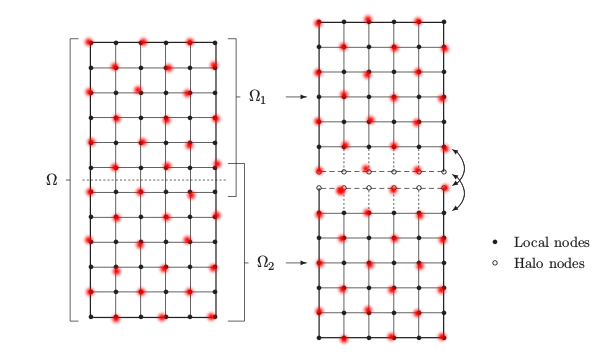
\includegraphics[width=\textwidth]{images/redblack.png}


Finally, the following performance model can be defined:

\[
S_p = \frac{T_{cr} + T_{cb} + T_{exr} + T_{exb}}{N_p}
\]

\begin{itemize}
  \item{$S_p$: Speedup}
  \item{$T_{cr}$: Red value computation}
  \item{$T_{exr}$: Red value halo exchange}
  \item{$T_{cb}$: Black value computation}
  \item{$T_{exb}$: Black value halo exchange}
  \item{$N_p$: Number of processor}
\end{itemize}

When $N_p = 1$\hspace{2em}$T_{exr} + T_{exb} \rightarrow 0$

\subsection{Parallel execution on Astral}

The main goal of high performance computing is to parallelize an algorithm to obtain results as fast
as possible. A parallel algorithm may be slower that the original algorithm if only one processor is
used, however this one is designed to able to reach high performance when it is running on multiplie
computational nodes. The speedup is probably the value the most interesting. It represents what is
the acceleration between 1-node computation and $N$-node computation. 

Two experience have been done on Astral, the same algorithm has been executed twice with a different
precision tolerance, the first one has been done with a low precision: $10^{-4}$ and the second with
a high precision: $10^{-6}$. Both of them have been run with 1, 2, 4, 8, 16 and 32 processors. The
algorithm used is Red-Black ordering Gauss-Seidel with a domain splitted in horizontal strips.

\subsubsection{Parallel execution with a low precision}

\input speedup

The speedup increase linearly, but it's slower than the optimal solution. Actually we could expect:

$$S_p = N_p$$

With
\begin{itemize}
  \item{$S_p$: Speedup}
  \item{$N_p$: Number of processors}
\end{itemize}

Instead of this perfect result, the speedup for $N_p = 32$ is only 17. This difference can be easily
explained. When there are more ndoes, there are more data exchanges. These are expensive and cost
a lot of time (processors cycles and networking latency). The above graph shows the aspects of the results,
underneath are some more detailled data.

\vspace{2em}
\hspace{-5em}
\begin{tabular}{l | c | c | c | c | c | c}
Number of processors & 1 & 2 & 4 & 8 & 16 & 32 \\
Execution time in seconds & 3506 & 2001 & 1019 & 602 & 356 & 201 \\
Number of iterations & 149,760 & 170,700 & 190530 & 216,360 & 249,360 & 289,980 \\
Speedup & 1 & 1.75 & 3.44 & 5.82 & 9.85 & 17.44 \\
Speedup evolution & - & $\times1.75$ & $\times1.96$ & $\times1.69$ & $\times1.69$  & $\times1.77$ \\
Difference with Optimal speedup & 0\% & 12.5\% & 14.0\% & 27.3\% & 38.4\% & 45.5\% \\
Average error with analytical & 10.5\% & 8.3\% & 6.6\% & 5.1\% & 3.8\% & 3.4\%
\end{tabular}
\captionof{table}{Data analysis of the obtained speedups with a $10^{-4}$ precision}
\vspace{1em}

The speedup evolution shows that its evolution is quite stable, not as fast as expected, but stable: $\approx 1.75$. However,
as this value is not two, we are going further and further from the optimal as it is illustrated by the difference with the linear speedup.

It is something to have a good speedup, but it's necessary to check if the results are good enough. All the previous figures have been done
with a mesh of $1024 \times 1024$. With this precision, the average error is really high. Having results which are 10\% different from the
analytical one is not acceptable. However, the more the number of processors, the lower the error to the analytical solution.
It can be explained by the way the stopping condition is implemented. The error is the sum the of all the local errors (of each subdomain),
so more the domain is divided, the slower it will reach the acceptance step. This is why there are much more iterations when the number of CPUs is getting bigger. 

\subsubsection{Parallel execution with a high precision}

The only difference in these results is the tolerance parameter, nothing else has changed.

\input speedup2

\vspace{2em}
\hspace{-5em}
\begin{tabular}{l | c | c | c | c | c | c}
Number of processors & 1 & 2 & 4 & 8 & 16 & 32 \\
Execution time in seconds & 18771 & 11101 & 5212 & 1923 & 1000 & 539 \\
Number of iterations & 591,330 & 629,250 & 660,510 & 696,150 & 735,450 & 779,010 \\
Speedup & 1 & 1.69 & 3.60 & 9.76 & 18.77 & 34.3 \\
Speedup evolution & - & $\times1.69$ & $\times2.13$ & $\times2.71$ & $\times1.92$  & $\times1.83$ \\
Difference with Optimal speedup & 0\% & -15.5\% & -10.0\% & +22.3\% & +17.3\% & +7.2\% \\
Average error with analytical & 0.22\% & 0.24\% & 0.44\% & 0.65\% & 1.55\% & 3.21\%
\end{tabular}
\captionof{table}{Data analysis of the obtained speedups with a $10^{-6}$ precision}
\vspace{1em}

In this case the results are particularly good, we reach a super-linear speedup. For 1, 2 and 4 processors,
the results are identical as the previous experience, the speedup is strongly increasing. ($> \times2$).

\vspace{1em}
These calculations are done with a higher precision, the logical consequence is that the whole computation
is longer, the number of iterations more important and mainly the average error compare to the analytical solution
is closer to 0, it is what we are expecting.

\vspace{1em}
How to explain such a high speedup: as we are using horizontal strips, the domain is decomposed in large horizontal subdomains.
With 32 processors it means, that each process is working on a $32\times1024$ matrix. The \textit{double} is 8 bytes long,
so each lines is weighting 8KB, and the matrix itself 256KB. The Astral HPC uses processors with 32KB of L1 cache and 4MB of
L2 cache, it means that the whole matrix can be store in them. There are no need to use the RAM. When the algorithm
is running on 1 CPU, the whole matrix can't fit in this cache and data exchanges from the RAM are necessary. Those slow down
the global operation.



\end{document}
